We implemented the event stream analytics solution presented in the previous chapter for an example use case. We wanted an interesting use case with diverse analytics possibilities that can be visualized well. Additionally, we wanted to use real data instead of mock data we generated ourselves, since real data are less predictable and can therefore better reveal real-world challenges of stream analytics. Smart and connected cities with public APIs provide an ideal source of streams since many different events occur in a system as complex as a city, and IoT facilitates digital access to these continuous streams in real time. Especially for public transportation many cities offer developers access to these data to integrate real-time information into, for example, route planning apps. Helsinki has one of the most mature public transportation API worldwide in terms of technology and documentation~\cite{AblyRealtime.2019}, therefore we will use its data as foundation for our use case.





\section{HSL Public Transportation APIs}
\gls{HSL} is the transportation authority for Helsinki and the surrounding municipalities. It oversees the operation of buses, trams, metros and overvehicles as well as ticket sale and inspection, but relies on third-party contractors for vehicle operation since it does not own any vehicles itself. HSL offers multiple publicly available APIs~\cite{HelsinkiRegionalTransportAuthority.2020b}:
\begin{itemize}
    \item High-frequency positioning (MQTT): vehicle positions every second, as well as events like arrivals at and departures from stops
    \item Routing (GraphQL): itinerary planning and information about stops and timetables
    \item Geocoding (HTTP): conversion between coordinates and places
    \item Map (HTTP): map images with points of interests
    \item Sales (HTTP): ticket sales and pricing information
\end{itemize}
We focus on the \gls{HFP} API since it provides us with a stream of real-time events, but we use other APIs to enrich events with more information.

The HFP API is accessible through a single MQTT broker~\cite{HelsinkiRegionalTransportAuthority.2020}. The topic structure allows subscription to specific event types, vehicle types and routes, but multiple/all can be selected by using wildcards. Following event types are available, among others:
\begin{itemize}
    \item Vehicle position (every second): geographical coordinates
    \item Vehicle has arrived at stop or departed from stop
    \item Vehicle's doors are being opened or closed
    \item Traffic light priority requests and responses
\end{itemize}
The JSON payload differs slightly between events, but usually contains an event timestamp, geographical coordinates (latitude and longitude), heading, speed, acceleration, as well as route and vehicle information. Some examples are shown in appendix~\ref{sec:appendix-input-events} Because vehicles are operated by different contractors, vehicles can only be uniquely identified by the combination of operator and vehicle number.

The volume of events over the course of a day is shown in figure~\ref{fig:usecase-hsl-daily-volume}. The volume is very low during the night and starts to increase after 05:00 with a first peak at 08:05 (1081 events per second). The volume remains steady until the second peak at 16:08 (1123 events per second), after which the volume slowly abates during the evening. This amounts to 58.4 million events per day.

The delay between events occuring in the real world (event timestamp) and the timestamp of arrival at the ingestion component over the course of a minute is shown in figure~\ref{fig:usecase-hsl-ingestion-lag}. Note that this is only partially the event-time skew/processing-time lag, since these metrics are defined using the timestamp of arrival at the \emph{processing} component. Most of the events actually have a negative delay, which is implausible since it would mean that events are ingested before they happen. This is probably due to clock synchronization issues between the vehicles and our system (we synchronize the system time of our EC2 instances using NTP as recommended by AWS). However, this does not affect correctnes or latency, since all processing is done in event time. Of more significance is the high tail delay, with some events only arriving after more than \SI{30}{\second}. This confirms the need for explicit event-time processing, where we can explicitly treat these events as late. With processing-time ordering, they would end up in the wrong window. 

\begin{figure}
	\centering
	\includegraphics[width=\textwidth]{plot_hsl_daily_event_volume}
	\caption[Daily event volume of the HSL HFP API]{Daily event volume of the HSL HFP API: the volume is the highest during rush hour}
	\label{fig:usecase-hsl-daily-volume}
\end{figure}

\begin{figure}
	\centering
	\includegraphics[width=\textwidth]{plot_hsl_ingestion_lag}
	\caption[Ingestion lag of the HSL HFP API]{Delay between the occurrence of events from the HSL HFP API and their arrival at the ingestion component over time (min: \SI{-542}{\milli\second}, median: \SI{-465}{\milli\second}, 90th percentile: \SI{-120}{\milli\second}, 99th percentile: \SI{9279}{\milli\second}, max: \SI{34684}{\milli\second})}
	\label{fig:usecase-hsl-ingestion-lag}
\end{figure}





\section{Analytics}
We decided on five analytics based on the HSL HFP data, visualized in figure~\ref{fig:usecase-analytics}. They cover different aspects of stream analytics and therefore allow us to evaluate multiple scenarios. All analytics jobs produce a stream that is produced to a separate Kafka topic. Most analytics divide the city of Helsinki into a grid of \emph{geocells} of equal size and calculate aggregates for each cell, resulting in a geographical distribution for the analytics when observing the results for all geocells.
\begin{description}
    \item[Vehicle distribution] Calculates the number of vehicles per geocell in the last \SI{30}{\second}, evaluated every \SI{5}{\second}. First, key the vehicle position stream by vehicle and apply a sliding window of \SI{30}{\second} evaluated every \SI{5}{\second} with a window evictor for duplicate events. This deduplication is necessary because each vehicle sends their position every second but we are only interested in the last position within the window, otherwise we would count each vehicle 30 times. Then, key the deduplicated stream by geocell and count the number of vehicles per geocell.
    \item[Delay distribution] Calculates delay statistics (median, 90th and 99th percentile) per geocell in the last \SI{5}{\minute}, evaluated every \SI{5}{\second}. First, calculate the difference between the scheduled and actual arrival on the arrival event stream in minutes (scheduled arrivals are only provided with minute resolution). Then, apply a sliding window of \SI{5}{\minute} evaluated every \SI{5}{\second} and calculate the statistics for all arrivals within the window. No deduplication is necessary.
    \item[Final stop distribution] Calculates the number of vehicles on a route with a final stop within a certain geocell per geocell in the last \SI{5}{\minute}, evaluated every \SI{5}{\second}. First, key the vehicle position stream by vehicle and apply a sliding window of \SI{5}{\minute} evaluated every \SI{5}{\second} with vehicle deduplication. Then, query the final stop of the route for each vehicle from the routing API using Flink asynchronous functions, since the final stop is not part of the event itself. All query responses are cached which drastically improves throughput and latency. The order of events is not maintained but can still be processed in event time by subsequent operators. Finally, key the stream of final stops by geocell and count the number of final stops per geocell.
    \item[Flow direction] Find the neighbor cell that the majority of vehicles move to per geocell in the last \SI{5}{\minute}, evaluated every \SI{5}{\second}. First, key the vehicle position stream by vehicle and apply a process function that only emits events when a vehicle changes the geocell. Then, key by origin cell and apply a sliding window of \SI{5}{\minute} evaluated every \SI{5}{\second} and find the neighbor cell which the most vehicles moved to. The result is a directed edge between two cells and the count of vehicles that traversed the edge within the window.
    \item[Emergency stop detection (stream)] Detect when vehicles brake quickly from cruising speed to a stop within \SI{10}{\second}. First, key the vehicle position stream by vehicle and use Flink's pattern recognition library to detect stops. The pattern requires vehicle to cruise at more than \SI{10}{\meter\per\second}, then decelerate and finally slow down to less than \SI{1}{\meter\per\second} within \SI{10}{\second}. For every detected stop, calculate the difference between the cruise speed and the speed after breaking as well as the maximum deceleration.
    \item[Emergency stop detection (table)] Does the same as the analytics above, but appends all events to a table using Flink's table API. The pattern is specified in SQL using the standardized \texttt{MATCH\_RECOGNIZE} clause, which uses Flink's streaming pattern recognition library under the hood. Finally, convert the detected stops and their speed difference and maximum deceleration back to a stream.
\end{description}
All analytics jobs use watermark-based completeness triggers and value output modes. Jobs that do not use deduplication have an allowed lateness equal to the window evaluation period (i.e. until the next window is complete), since later data would not be displayed in the visualization component according to the second policy. Jobs with deduplication do not have late triggers since they do not work well with eviction and multiple subsequent windows.

\begin{figure}
    \centering
	\begin{subfigure}[c]{0.30\textwidth}
        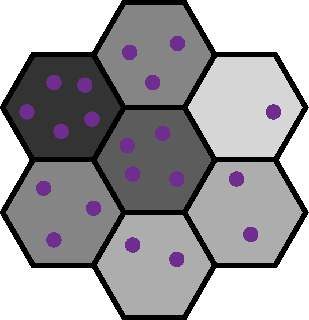
\includegraphics[width=\textwidth]{usecase_analytics_vehicledist}%
		\subcaption{Vehicle distribution}
    \end{subfigure}%
    \hfill
	\begin{subfigure}[c]{0.30\textwidth}
        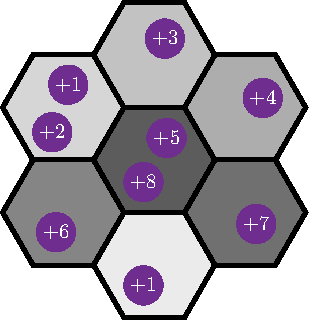
\includegraphics[width=\textwidth]{usecase_analytics_delaydist}%
		\subcaption{Delay distribution}
	\end{subfigure}%
    \hfill
	\begin{subfigure}[c]{0.30\textwidth}
        \centering
        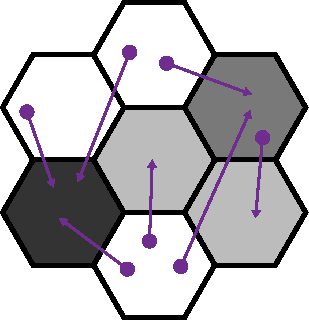
\includegraphics[width=\textwidth]{usecase_analytics_finalstopdist}%
		\subcaption{Final stop distribution}
    \end{subfigure}
    
    \bigskip
    
	\begin{subfigure}[c]{0.30\textwidth}
        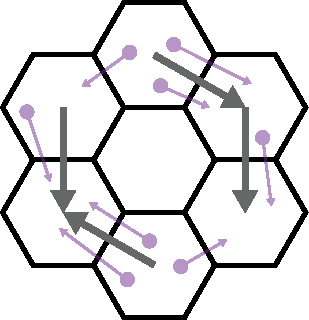
\includegraphics[width=\textwidth]{usecase_analytics_flowdir}%
		\subcaption{Flow direction}
	\end{subfigure}%
    \hfill
	\begin{subfigure}[c]{0.60\textwidth}
		\includegraphics[width=\textwidth]{plot_usecase_analytics_emergency_stop}%
		\subcaption{Emergency stop detection}
	\end{subfigure}
	\caption{Analytics for public transportation}
	\label{fig:usecase-analytics}
\end{figure}



\subsection{Geocells}
To support analytics that calculate aggregations (like vehicle distributions) over discrete geographical regions, a discrete global grid system is required which can partition the continuous space of geographical coordinates into geocells. While this grid can be defined based on data like postal codes, regular grid systems with even distribution are desirable for most applications~\cite[p.~121]{Sahr.2003}. There are many approaches to reduce distortion introduced by applying a regular two-dimensional grid onto the three-dimensional sphere of the earth. We use Uber's H3\footnote{\url{https://h3geo.org/}} library, which first projects the earth's surface onto an icosahedron and then overlays a grid of 122 hexagonal base cells (pentagons need to be used at vertices, but these are deliberately located in the water to reduce error). Each base cell has an average edge length of \SI{1108}{\kilo\metre}, but can be recursively sub-divided into seven smaller cells. At the finest resolution, the average edge length is only \SI{50}{\centi\metre}. The choice of hexagons over triangles and squares (the only other two regular polygons that tile perfectly) simplifies motion analysis, since the distance between the center of a hexagon and the center of is hexagons is the same on all sides, compared to two different distances for squares and three for triangles. This enables easy approximation of distances and radii through the number of cells between two points. For a more detailed description of H3, refer to~\cite{Brodsky.2018}.

H3 has bindings for all languages that we use in our solution (Java, Python and JavaScript). This enables us to use geocells in analytics jobs and then draw the according cells on a map for visualization. At the resolution that we use, the globe is divided into 4,800,000,000 geocells with an average edge length of \SI{174}{\metre} and an average outer diameter of \SI{348}{\metre}.



\section{Data Flow Example}
\label{sec:usecase-dataflow}
To better understand the data flow through and interaction of components of our solution, we now look at an end-to-end example and trace the route of a vehicle position event from the HFP API until its visualization as part of the vehicle distribution job. Use the architecture from figure~\ref{fig:solution-architecture} as reference.

The ingestion component is the component interfacing with the HSL MQTT broker. When it is first started, the component creates an MQTT connector which subscribes to the \texttt{/hfp/v2/journey/ongoing/vp/\#} topic to receive vehicle positions (the \texttt{\#} is a wildcard supported by the HSL broker since the actual topic is much more elaborate). An example of a vehicle position event as it is produced by the MQTT API is shown in listing~\ref{lst:appendix-event-vp-raw}. This event is processed by the respective processor which extracts the event timestamp and all other relevant information to build a protobuf message. This message is then wrapped in the common event schema and serialized. While we normally use the much more compact binary format (\SI{150}{\byte} on average), the JSON variant shown in listing~\ref{lst:appendix-event-vp-protobuf} (\SI{450}{\byte} on average using UTF-8 without indentation) is very useful for debugging and can be used interchangeably (compare with the schema definition from listing~\ref{lst:solution-protobuf-event-schema}). Note how the message contains the nested type, which enables type-safe deserialization, and the ingestion timestamp is added. The event leaves the ingestion component when it is written to the Kafka topic \texttt{input.vehicle-position} for all vehicle position events. Examples for all three input event types that we use (vehicle position, arrival, departure) can be found in appendix~\ref{sec:appendix-input-events}.

The processing component runs all stream analytics jobs. The Flink definition for the vehicle distribution job is shown in listing~\ref{lst:usecase-vehicle-distribution-job} (most referenced methods and classes are custom but not shown for clarity). The vehicle position Kafka topic as well as the expected class for protobuf messages is declared in line 1. Then the stream is keyed by vehicle, which partitions the stream and results in shuffling to bring the events to the appropriate task slot (in case of a parallelism larger than 1). This might add network latency if the task slot is located in a task manager on another node. The keyed stream is then windowed into sliding \SI{30}{\second} windows which are evaluated every \SI{5}{\second}. This means that every vehicle position event will be part of 6 window instances. The window is only triggered once on-time when the watermark for the window event passes. We use bounded-out-of-orderness watermarking of \SI{1}{\second}. Since the vehicle position event happens at 08:24:36, the window is evaluated when the first event with an event timestamp of 08:24:37 is observed (all timestamps are in UTC, which is 3 hours ahead of Helsinki time). We apply deduplication at evaluation to only retain the most recent vehicle position event for each vehicle within the window. The transformation of the window is an identity function that emits all events as-is (apart from adjusting the event timestamp to the end of the window). This is required so the stream can be re-shuffled in the next step, where we key the stream by geocell. \\ This results in partitions where all events within a partition occurred in the same geocell. Since we already applied a sliding window which emits its contents every \SI{5}{\second} with adjusted event timestamps, we only need a tumbling window the length of the slide period. Note we still calculate the distribution over the last \SI{30}{\second}. The second window is aggregated eagerly using an \javainline/AggregationFunction/. Finally, the result shown in listing~\ref{lst:usecase-analytics-protobuf} is emitted to the Kafka topic \texttt{analytics.vehicle-distribution}. The result shows the number of vehicles in the same geocell as our example vehicle for the window from 08:24:20 to 08:24:50. When executing this job on a Flink cluster, the framework automatically handles the distributed and fault-tolerant execution with event-time ordering.

\begin{listing}
\inputminted{java}{code/usecase_vehicle_distribution_job.java}
\caption{Job definition for vehicle distribution analytics}
\label{lst:usecase-vehicle-distribution-job}
\end{listing}

\begin{listing}
\inputminted{json}{code/usecase_analytics_protobuf.json}
\caption{Vehicle distribution result as protobuf message}
\label{lst:usecase-analytics-protobuf}
\end{listing}

The visualization component shows the vehicle distribution to the user. The backend consumes the vehicle distribution results Kafka topic and converts all protobuf messages to a JSON string and forwards them to the frontend using Socket.IO. The conversion eliminates the need for integrating the protobuf definitions into the frontend. When the user loads the frontend website, it establishes a connection to the Socket.IO server using HTTP or WebSockets. Once the analytics results arrive, the frontend uses H3 to calculate the hexagon outline of the hexagon and draws it on the map as shown in figure~\ref{fig:usecase-map}. Because each hexagon is shaded according to the vehicle count, looking at all geocells gives an impression of the vehicle distribution in real time. All results are invalidated after \SI{10}{\second} and the associated hexagon is removed from the map if no updates for that geocell arrived within that time. This can be the case for regions that are not very busy, since results for a geocell are only produced if there are vehicles within it. The total time is takes from the position measurement of a vehicle until a result based on that measurement is shown in the visualization component can be as low as \SI{3}{\second}. 

\begin{figure}
	\centering
    % \includegraphics[width=\textwidth]{plot_hsl_daily_event_volume}
    FIGURE OF VISUALIZATION MAP
    \caption[Visualization on map with geocells]{Visualization on map with geocells: each geocell is shaded according to its vehicle count in real-time}
    \label{fig:usecase-map}
\end{figure}
